\begin{figure*}[t]
    \begin{subfigure}{0.3\textwidth}
        \centering
        \resizebox{\linewidth}{!}{
            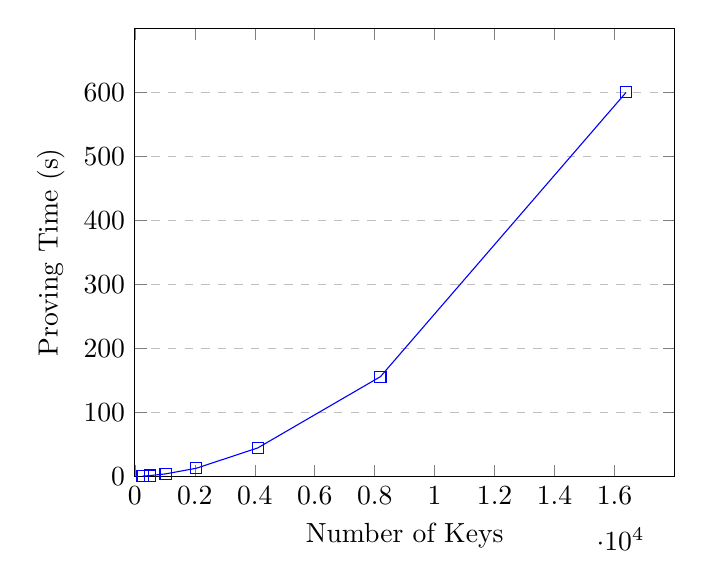
\begin{tikzpicture}
                \begin{axis}[
                    xlabel={Number of Keys},
                    ylabel={Proving Time (s)},
                    xmin=0,xmax=18000,
                    ymin=0,ymax=700,
                    xtick={0,2000,4000,6000,8000,10000,12000,14000,16000},
                    ytick={0,100,200,300,400,500,600},
                    ymajorgrids=true,
                    grid style=dashed,
                ]
                \addplot[
                    color=blue,
                    mark=square,
                ]
                    coordinates {
                        (256,0.63)(512,1.48)(1024,4.11)(2048,12.9)(4096,44.59)(8192,155.94)(16384,599.78)
                    };
                \end{axis}
            \end{tikzpicture}
        }
        \subcaption{}
    \end{subfigure}
    \begin{subfigure}{0.3\textwidth}
        \centering
        \resizebox{\linewidth}{!}{
            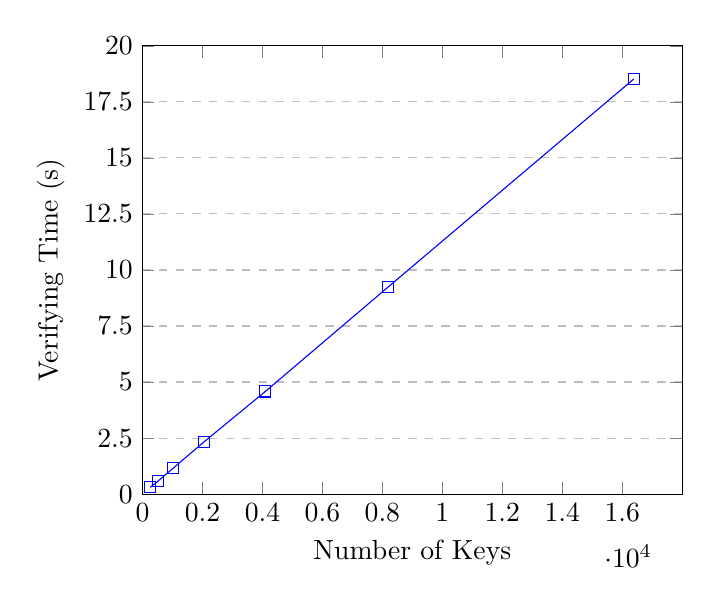
\begin{tikzpicture}
                \begin{axis}[
                    xlabel={Number of Keys},
                    ylabel={Verifying Time (s)},
                    xmin=0,xmax=18000,
                    ymin=0,ymax=20,
                    xtick={0,2000,4000,6000,8000,10000,12000,14000,16000},
                    ytick={0,2.5,5,7.5,10,12.5,15,17.5,20},
                    ymajorgrids=true,
                    grid style=dashed,
                ]
                \addplot[
                    color=blue,
                    mark=square,
                ]
                    coordinates {
                        (256,0.3)(512,0.58)(1024,1.16)(2048,2.33)(4096,4.58)(8192,9.24)(16384,18.52)
                    };
                \end{axis}
            \end{tikzpicture}
        }
        \subcaption{}
    \end{subfigure}
    \begin{subfigure}{0.3\textwidth}
        \centering
        \resizebox{\linewidth}{!}{
            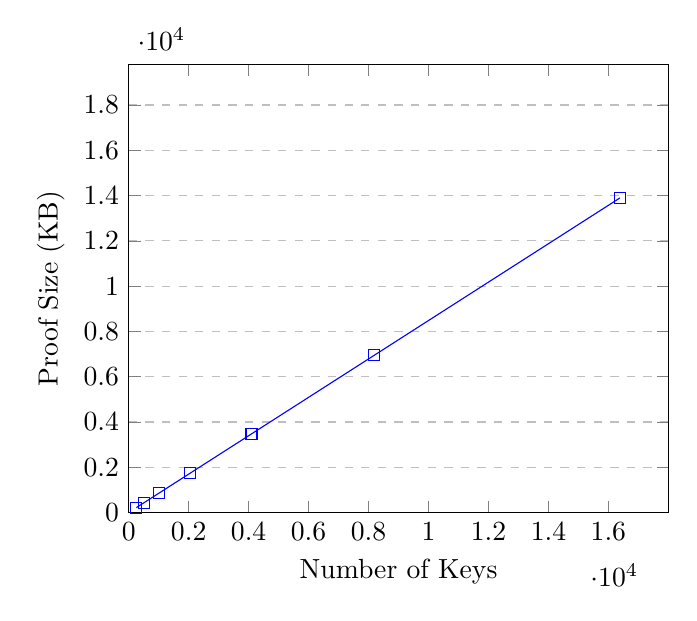
\begin{tikzpicture}
                \begin{axis}[
                    xlabel={Number of Keys},
                    ylabel={Proof Size (KB)},
                    xmin=0,xmax=18000,
                    ymin=0,ymax=19800,
                    xtick={0,2000,4000,6000,8000,10000,12000,14000,16000},
                    ytick={0,2000,4000,6000,8000,10000,12000,14000,16000,18000,20000},
                    ymajorgrids=true,
                    grid style=dashed,
                ]
                \addplot[
                    color=blue,
                    mark=square,
                ]
                    coordinates {
                        (256,217.0)(512,434.0)(1024,868.0)(2048,1736.0)(4096,3473.0)(8192,6946.0)(16384,13893.0)
                    };
                \end{axis}
            \end{tikzpicture}
        }
        \subcaption{}
    \end{subfigure}
\caption{Performance of \bootstrap}
\label{fig:keys}
\end{figure*}

\begin{figure*}[t]
    \begin{subfigure}{0.3\textwidth}
        \resizebox{\linewidth}{!}{
            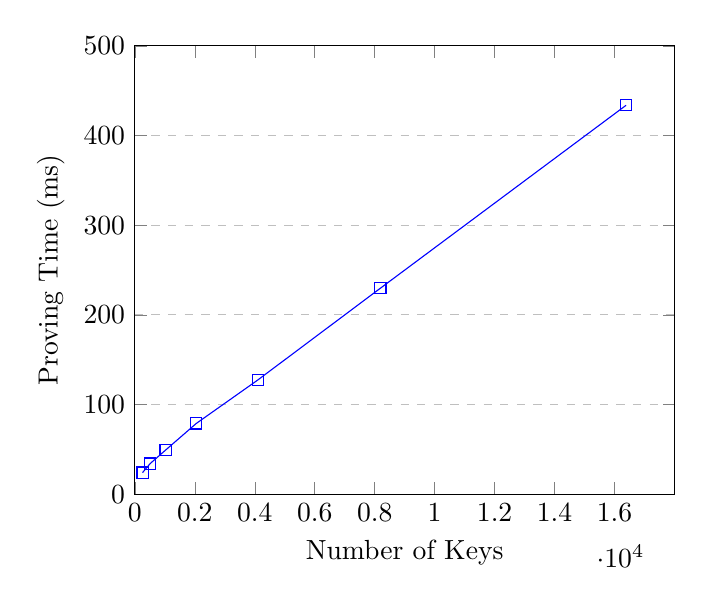
\begin{tikzpicture}
                \begin{axis}[
                    xlabel={Number of Keys},
                    ylabel={Proving Time (ms)},
                    xmin=0,xmax=18000,
                    ymin=0,ymax=500,
                    xtick={0,2000,4000,6000,8000,10000,12000,14000,16000},
                    ytick={0,100,200,300,400,500},
                    ymajorgrids=true,
                    grid style=dashed,
                ]
                \addplot[
                    color=blue,
                    mark=square,
                ]
                    coordinates {
                        (256,24.02)(512,34.1)(1024,49.09)(2048,78.8)(4096,127.17)(8192,229.71)(16384,433.66)
                    };
                \end{axis}
            \end{tikzpicture}
        }
        \subcaption{}
    \end{subfigure}
    \begin{subfigure}{0.3\textwidth}
        \resizebox{\linewidth}{!}{
            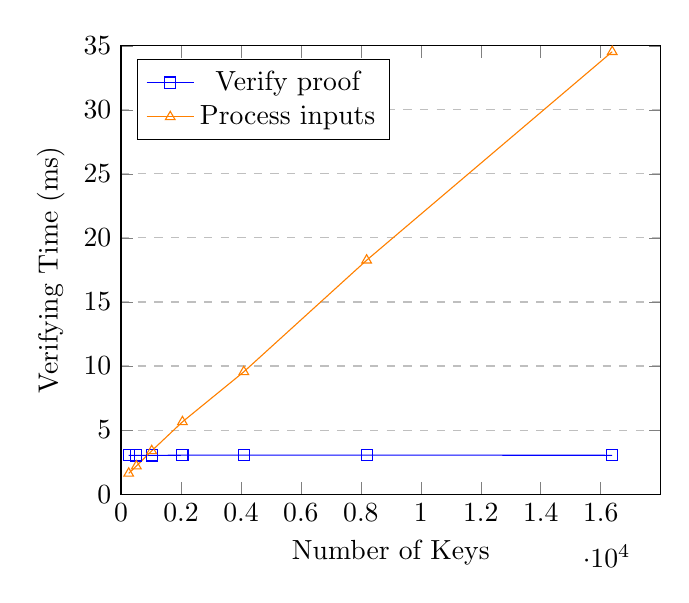
\begin{tikzpicture}
                \begin{axis}[
                    xlabel={Number of Keys},
                    ylabel={Verifying Time (ms)},
                    xmin=0,xmax=18000,
                    ymin=0,ymax=35,
                    xtick={0,2000,4000,6000,8000,10000,12000,14000,16000},
                    ytick={0,5,10,15,20,25,30,35},
                    ymajorgrids=true,
                    grid style=dashed,
                    legend pos=north west,
                ]
                \addplot[
                    color=blue,
                    mark=square,
                ]
                    coordinates {
                        (256,3.03)(512,3.02)(1024,3.02)(2048,3.04)(4096,3.04)(8192,3.05)(16384,3.03)
                    };
                \addlegendentry{Verify proof}

                \addplot[
                    color=orange,
                    mark=triangle,
                ]
                    coordinates {
                        (256,1.62)(512,2.19)(1024,3.38)(2048,5.64)(4096,9.55)(8192,18.26)(16384,34.54)
                    };
                \addlegendentry{Process inputs}
                \end{axis}
            \end{tikzpicture}
        }
        \subcaption{}
    \end{subfigure}
    \begin{subfigure}{0.3\textwidth}
        \resizebox{\linewidth}{!}{
            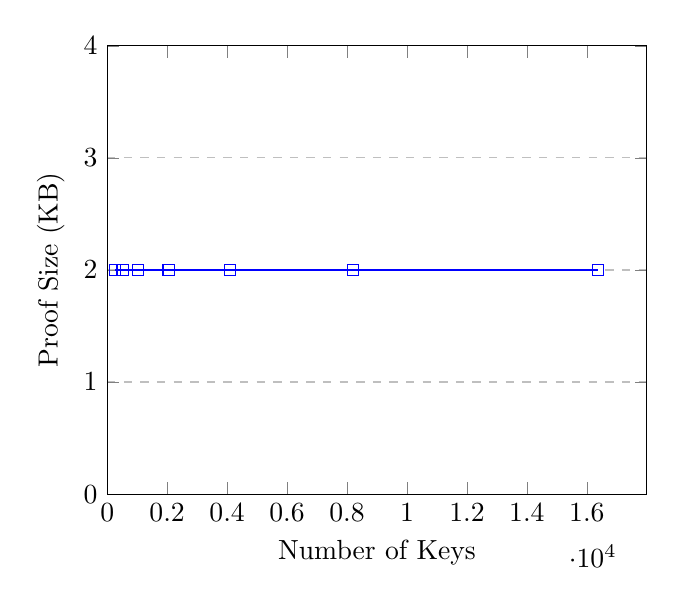
\begin{tikzpicture}
                \begin{axis}[
                    xlabel={Number of Keys},
                    ylabel={Proof Size (KB)},
                    xmin=0,xmax=18000,
                    ymin=0,ymax=4,
                    xtick={0,2000,4000,6000,8000,10000,12000,14000,16000},
                    ytick={0,1,2,3,4},
                    ymajorgrids=true,
                    grid style=dashed,
                ]
                \addplot[
                    color=blue,
                    mark=square,
                ]
                    coordinates {
                        (256,2.0)(512,2.0)(1024,2.0)(2048,2.0)(4096,2.0)(8192,2.0)(16384,2.0)
                    };
                \end{axis}
            \end{tikzpicture}
        }
        \subcaption{}
    \end{subfigure}
\caption{Performance of \poa}
\label{fig:poa}
\end{figure*}

\begin{figure*}[t]
    \begin{subfigure}{0.3\textwidth}
        \resizebox{\linewidth}{!}{
            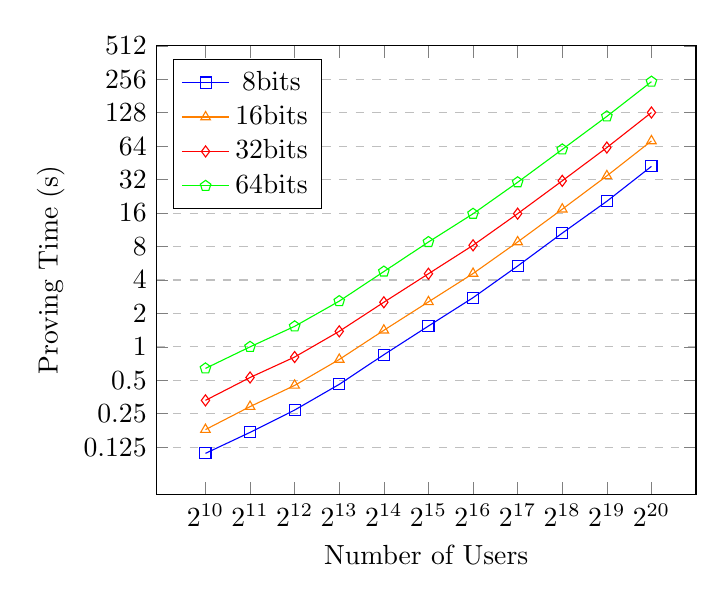
\begin{tikzpicture}
                \begin{loglogaxis}[
                    xlabel={Number of Users},
                    ylabel={Proving Time (s)},
                    xmin=0,xmax=2097152,
                    ymin=0,ymax=512,
                    xtick={0,1024,2048,4096,8192,16384,32768,65536,131072,262144,524288,1048576},
                    ytick={0,0.125,0.25,0.5,1,2,4,8,16,32,64,128,256,512},
                    xticklabels={$2^{10}$,$2^{11}$,$2^{12}$,$2^{13}$,$2^{14}$,$2^{15}$,$2^{16}$,$2^{17}$,$2^{18}$,$2^{19}$,$2^{20}$},
                    yticklabels={0.125,0.25,0.5,1,2,4,8,16,32,64,128,256,512},
                    ymajorgrids=true,
                    grid style=dashed,
                    legend pos=north west,
                ]
                \addplot[
                    color=blue,
                    mark=square,
                ]
                    coordinates {
                        (1024,0.11)(2048,0.17)(4096,0.27)(8192,0.46)(16384,0.85)(32768,1.54)(65536,2.77)(131072,5.34)(262144,10.56)(524288,20.43)(1048576,42.1)
                    };
                \addlegendentry{8bits}

                \addplot[
                    color=orange,
                    mark=triangle,
                ]
                    coordinates {
                        (1024,0.18)(2048,0.29)(4096,0.45)(8192,0.77)(16384,1.41)(32768,2.54)(65536,4.57)(131072,8.79)(262144,17.33)(524288,34.56)(1048576,71.31)
                    };
                \addlegendentry{16bits}

                \addplot[
                    color=red,
                    mark=diamond,
                ]
                    coordinates {
                        (1024,0.33)(2048,0.53)(4096,0.81)(8192,1.38)(16384,2.52)(32768,4.55)(65536,8.2)(131072,15.8)(262144,31.19)(524288,62.16)(1048576,128.49)
                    };
                \addlegendentry{32bits}

                \addplot[
                    color=green,
                    mark=pentagon,
                ]
                    coordinates {
                        (1024,0.64)(2048,1.0)(4096,1.53)(8192,2.58)(16384,4.76)(32768,8.78)(65536,15.76)(131072,30.27)(262144,59.8)(524288,118.57)(1048576,243.53)
                    };
                \addlegendentry{64bits}

                \end{loglogaxis}
            \end{tikzpicture}
        }
        \subcaption{}
    \end{subfigure}
    \begin{subfigure}{0.3\textwidth}
        \resizebox{\linewidth}{!}{
            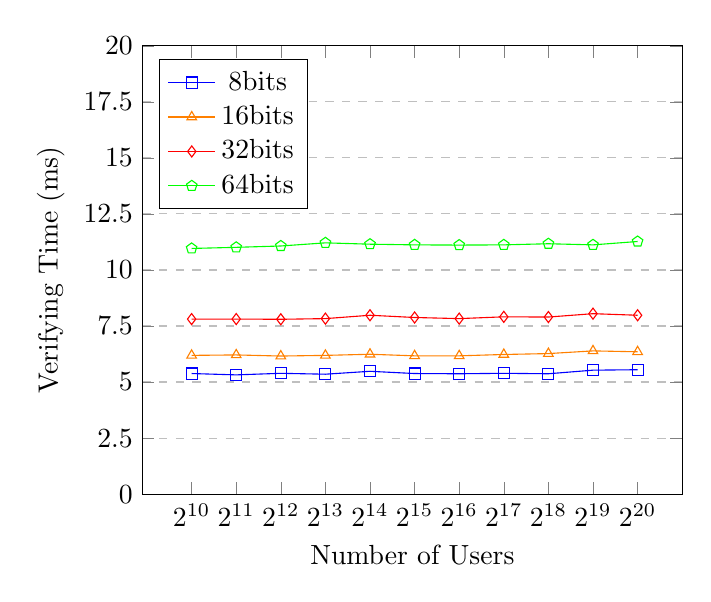
\begin{tikzpicture}
                \begin{semilogxaxis}[
                    xlabel={Number of Users},
                    ylabel={Verifying Time (ms)},
                    xmin=0,xmax=2097152,
                    ymin=0,ymax=20.0,
                    xtick={0,1024,2048,4096,8192,16384,32768,65536,131072,262144,524288,1048576},
                    ytick={0,2.5,5.0,7.5,10.0,12.5,15.0,17.5,20.0},
                    xticklabels={$2^{10}$,$2^{11}$,$2^{12}$,$2^{13}$,$2^{14}$,$2^{15}$,$2^{16}$,$2^{17}$,$2^{18}$,$2^{19}$,$2^{20}$},
                    ymajorgrids=true,
                    grid style=dashed,
                    legend pos=north west,
                ]

                \addplot[
                    color=blue,
                    mark=square,
                ]
                    coordinates {
                        (1024,5.38)(2048,5.32)(4096,5.39)(8192,5.35)(16384,5.48)(32768,5.38)(65536,5.37)(131072,5.39)(262144,5.37)(524288,5.53)(1048576,5.55)
                    };
                \addlegendentry{8bits}

                \addplot[
                    color=orange,
                    mark=triangle,
                ]
                    coordinates {
                        (1024,6.19)(2048,6.21)(4096,6.16)(8192,6.19)(16384,6.24)(32768,6.17)(65536,6.17)(131072,6.23)(262144,6.27)(524288,6.39)(1048576,6.35)
                    };
                \addlegendentry{16bits}

                \addplot[
                    color=red,
                    mark=diamond,
                ]
                    coordinates {
                        (1024,7.81)(2048,7.81)(4096,7.8)(8192,7.83)(16384,7.98)(32768,7.88)(65536,7.83)(131072,7.91)(262144,7.9)(524288,8.05)(1048576,7.98)
                    };
                \addlegendentry{32bits}

                \addplot[
                    color=green,
                    mark=pentagon,
                ]
                    coordinates {
                        (1024,10.96)(2048,11.01)(4096,11.07)(8192,11.21)(16384,11.15)(32768,11.12)(65536,11.11)(131072,11.12)(262144,11.17)(524288,11.12)(1048576,11.27)
                    };
                \addlegendentry{64bits}

                \end{semilogxaxis}
            \end{tikzpicture}
        }
        \subcaption{}
    \end{subfigure}
    \begin{subfigure}{0.3\textwidth}
        \resizebox{\linewidth}{!}{
            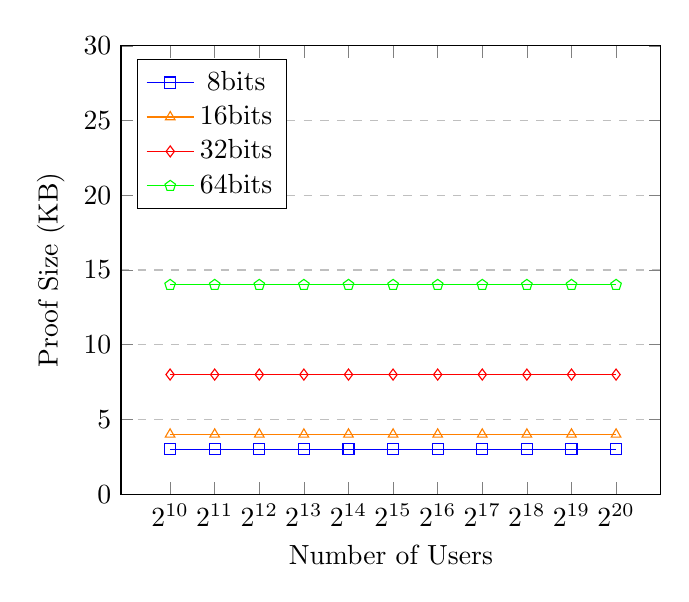
\begin{tikzpicture}
                \begin{semilogxaxis}[
                    xlabel={Number of Users},
                    ylabel={Proof Size (KB)},
                    xmin=0,xmax=2097152,
                    ymin=0,ymax=30,
                    xtick={0,1024,2048,4096,8192,16384,32768,65536,131072,262144,524288,1048576},
                    ytick={0,5,10,15,20,25,30},
                    xticklabels={$2^{10}$,$2^{11}$,$2^{12}$,$2^{13}$,$2^{14}$,$2^{15}$,$2^{16}$,$2^{17}$,$2^{18}$,$2^{19}$,$2^{20}$},
                    ymajorgrids=true,
                    grid style=dashed,
                    legend pos=north west,
                ]

                \addplot[
                    color=blue,
                    mark=square,
                ]
                    coordinates {
                        (1024,3.0)(2048,3.0)(4096,3.0)(8192,3.0)(16384,3.0)(32768,3.0)(65536,3.0)(131072,3.0)(262144,3.0)(524288,3.0)(1048576,3.0)
                    };
                \addlegendentry{8bits}

                \addplot[
                    color=orange,
                    mark=triangle,
                ]
                    coordinates {
                        (1024,4.0)(2048,4.0)(4096,4.0)(8192,4.0)(16384,4.0)(32768,4.0)(65536,4.0)(131072,4.0)(262144,4.0)(524288,4.0)(1048576,4.0)
                    };
                \addlegendentry{16bits}

                \addplot[
                    color=red,
                    mark=diamond,
                ]
                    coordinates {
                        (1024,8.0)(2048,8.0)(4096,8.0)(8192,8.0)(16384,8.0)(32768,8.0)(65536,8.0)(131072,8.0)(262144,8.0)(524288,8.0)(1048576,8.0)
                    };
                \addlegendentry{32bits}

                \addplot[
                    color=green,
                    mark=pentagon,
                ]
                    coordinates {
                        (1024,14.0)(2048,14.0)(4096,14.0)(8192,14.0)(16384,14.0)(32768,14.0)(65536,14.0)(131072,14.0)(262144,14.0)(524288,14.0)(1048576,14.0)
                    };
                \addlegendentry{64bits}

                \end{semilogxaxis}
            \end{tikzpicture}
        }
        \subcaption{}
    \end{subfigure}
\caption{Performance of \pol}
\label{fig:pol}
\end{figure*}
